\begin{figure}[htbp]
    \centering

    \begin{subfigure}[t]{0.45\linewidth}
        \centering
        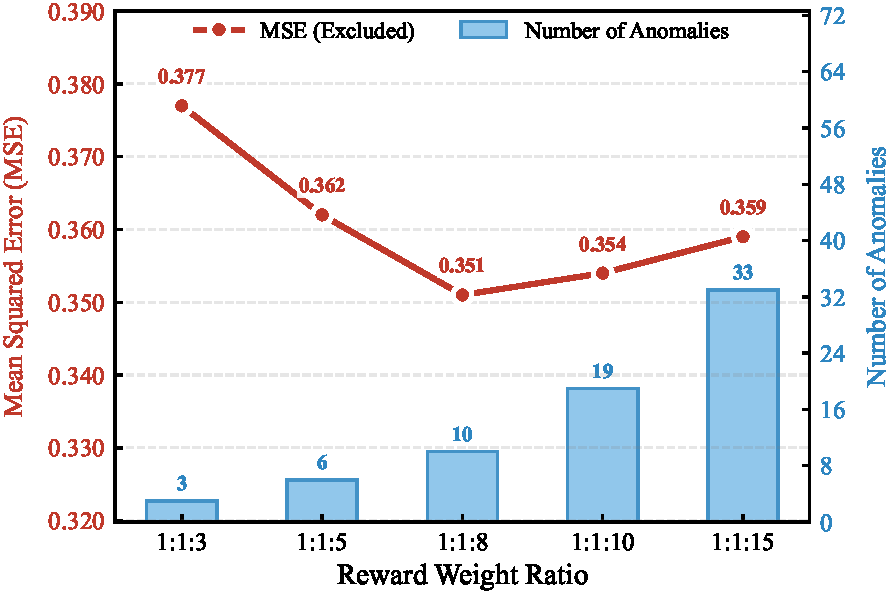
\includegraphics[width=\linewidth]{figures/ablation/ablation01.pdf}
        \caption{Impact of the reward weight ratio.}
        \label{fig:ablation_01}
    \end{subfigure}
    \hfill
    \begin{subfigure}[t]{0.52\linewidth}
        \centering
        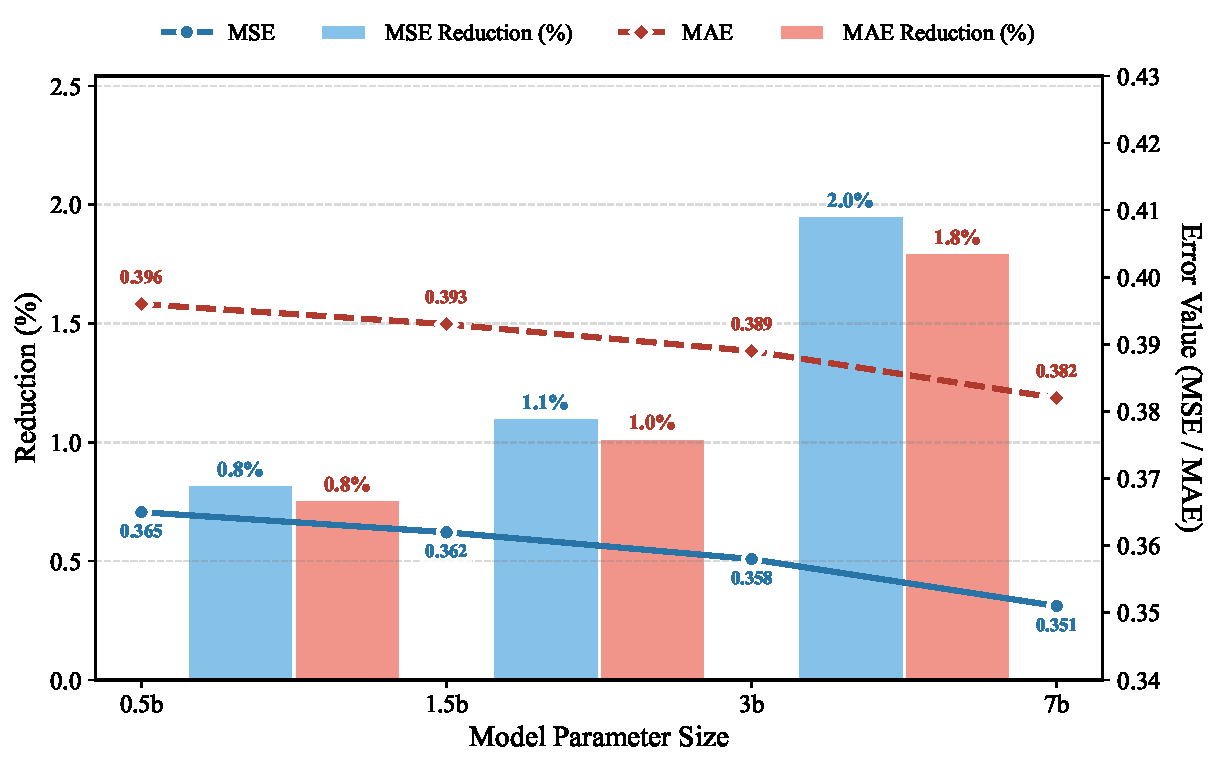
\includegraphics[width=\linewidth]{figures/ablation/ablation03_combined.pdf}
        \caption{Scaling laws on training efficiency and forecasting performance.}
        \label{fig:ablation_03}
    \end{subfigure}


    \caption{Ablation analysis of reward weighting and model scaling. Left: the red line represents the Mean Squared Error (MSE) on the excluded dataset, while the blue bars indicate the number of detected anomalies. Right: the line chart tracks MSE and MAE, showing that increased model capacity leads to consistent improvements in prediction accuracy.}
    \label{fig:ablation_combined}

\end{figure}
